\documentclass{article}
\usepackage[utf8]{inputenc}
\usepackage[T1]{fontenc}
\usepackage{amsmath}
\usepackage{url}
\usepackage{listings}
\usepackage{xcolor}
\usepackage{graphicx}
\usepackage{parskip}
\usepackage[toc,page]{appendix}

\definecolor{codegreen}{rgb}{0,0.6,0}
\definecolor{codegray}{rgb}{0.5,0.5,0.5}
\definecolor{codepurple}{rgb}{0.58,0,0.82}
\definecolor{backcolour}{rgb}{0.95,0.95,0.92}

\lstdefinestyle{mystyle}{
    backgroundcolor=\color{backcolour},   
    commentstyle=\color{codegreen},
    keywordstyle=\color{magenta},
    numberstyle=\tiny\color{codegray},
    stringstyle=\color{codepurple},
    basicstyle=\ttfamily\footnotesize,
    breakatwhitespace=false,         
    breaklines=true,                 
    captionpos=b,                    
    keepspaces=true,                 
    numbers=left,                    
    numbersep=5pt,                  
    showspaces=false,                
    showstringspaces=false,
    showtabs=false,                  
    tabsize=2
}
\lstset{style=mystyle}

\author{Wenhao LUO}
\title{Rapport du projet IA échecs}
\begin{document}
\maketitle
\date{}

\cleardoublepage
\tableofcontents

\clearpage

\section{Introduction}
\par En suivant le cours \textbf{8INF878-Intelligence Artificielle} de l'Université de Québec à Chicoutimi, on a réalisé ce projet "compétition d'agent intelligents pour le jeu d'échecs" par l'implémentation d'une intelligence artificielle comme un engine jouable sur la plateforme ARENA.

\par Ce document sert à introduire le fonctionnement de ce programme, à expliquer comment on a réalisé cette implémentation et à discuter les difficultés rencontrés pendant la réalisation de ce projet.

\section{Fonctionnement du programme}

\subsection{Informations générales}
\par Le programme réalisé, nommé \texttt{OCAP} est un engine qui est capable de jouer le jeu d'échecs avec l'aide du logiciel ARENA. Il est capable de comprendre une partie des commandes définies avec le protocole UCI, qui le permet de reconstituer, d'analyser et de jouer un jeu d'échecs avec les données transmis par \texttt{stdin} et \texttt{stdout}.

\subsection{Commandes acceptées} \label{commandes}
\par Voici la liste de toutes les commandes qui peuvent être insérées et comprises par ce logiciel :
\begin{itemize}
    \item \texttt{uci} : en acceptant cette commande, le programme retourne son identifiant et son auteur ;
    \item \texttt{isready} : en acceptant cette commande, le programme retourne le message "isready" qui permet de confirmer qu'il est prêt au calcul ;
    \item \texttt{go} : en acceptant cette commande, le programme commence à effectuer les calculs ; il devra retourner un résultat plus tard avec un délai prédéfini ;
    \item \texttt{stop} : en acceptant cette commande, le programme arrête son calcul et il retourne un résultat le plus vite possible ;
    \item \texttt{quit} : en acceptant cette commande, le programme arrête son fonctionnement et termine l'exécution de tous les threads ;
    \item \texttt{position startpos [moves] <move1>, <move2>, ...} : en acceptant cette commande, le programme reconstitue un damier au sein du programme, qui permet de réaliser les calculs plus tard.
\end{itemize}

\subsection{Interaction avec ce programme}
\par Avec l'interface ARENA, une personne peut jouer un jeu d'échecs avec ce programme en le chargeant comme un des engines de l'ARENA. C'est également possible de jouer le jeu directement en lançant ce programme dans une ligne de commande par insérer les commandes listées dans la section \ref{commandes}.


\section{Implémentation}

\subsection{Langage et paradigme utilisé}
\par Le programme est écrit en Java, et naturellement avec le paradigme OOP. Certaines parties sont écrites avec multithreading.

\subsection{Topologie du programme}
\par Le programme peut être séparé en trois parties différentes :
\begin{itemize}
    \item un damier et des pièces de l'échecs construct au sein du système, qui permet de reconstruire un scénario du jeu et l'évaluer ;
    \item un programme qui permet d'analyser le meilleur choix dans une situation donnée, et de prendre des décisions ;
    \item un parseur minimise qui permet de comprendre les commandées entrées et de communiquer avec les autres composantes du programme.
\end{itemize}

\par Prochainement on va parler des trois parties à l'ordre.

\subsection{Damier et pièces}
\par La première partie du programme réalise un damier de l'échecs \texttt{Board} avec des pièces qui peuvent être mises sur un damier. Un damier contient une liste de pièces et leur coordonnées, qui est un "état" du jeu. J'ai également implémenté les fonctions qui permettent de réaliser les fonctionnements basiques, comme une fonction qui retrouve une liste des actions légales, et une autre fonction qui permet de réaliser une transition entre deux états. Les exemples peuvent être retrouvés dans le listing \ref{lst:board}.

\par Des pièces du jeu sont programmés avec un héritage de classe : toutes les pièces sont considérées comme un membre de la classe \texttt{Piece}, ensuite chaque pièce réalise ses propres méthodes. Le code de la classe \texttt{Piece} est disponible comme le listing \ref{lst:piece}.

\par Le problème de gestion de mémoire a été pris en compte pendant le développement. Notons que dans la classe \texttt{Board} les pièces ne sauvegardent pas leur position sur le damier ; en fait il ne sauvegarde non plus l'objet \texttt{Board}. J'ai choisi cette implémentation afin d'éviter de recopier les objets \texttt{Piece} entre la transition des deux damiers.

\par Si un nouveau état du jeu doit être créé en déplaçant une pièce sur un damier, alors seulement la position des pièces sera modifié ; les différents damiers partagent les mêmes pièces : chaque fois on trace la position des pièces par un nouveau dictionnaire et tous les dictionnaires pointent les mêmes objets. Une illustration est donnée comme le figure \ref{fig:copies}.

\begin{figure}[htb]
    \centering
    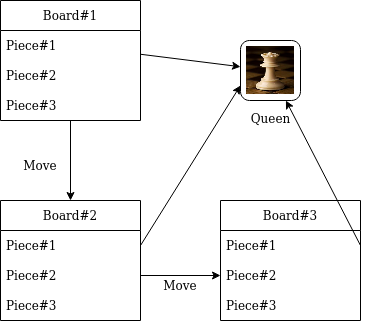
\includegraphics[width = 0.7\linewidth]{illustation.png}
    \caption{Illustration sur la création des nouveaux états.}
    \label{fig:copies}
\end{figure}

\par La classe \texttt{Board} génère toutes les possibles actions à partir des positions des pièces. Les actions sont nommées comme \texttt{Move}. Un damier peut généré un nouveau damier selon une instance de \texttt{Move} donnée. On est donc capable de décrire les différents états et leur transition.

\subsection{Analyseur}
\subsubsection{Algorithme utilisé}
\par On utilise une recherche en appliquant un algorithme élagage alpha-bêta\cite{enwiki:Alphabeta}. Le principe de cet algorithme est d'explorer les différents nœuds par profondeur, en applicant une optimisation supplémentaire en mémorisant deux valeurs $\alpha$ et $\beta$. Ces valeurs représentent les meilleurs/pires cas possibles. Si le résultat retrouvé par un nœud dépasse ces valeurs, alors théoriquement ces nœuds seront jamais visités, supposant que les joueurs ne choisissent que les meilleurs choix. Ainsi on évite de faire les visites non nécessaires.

\subsubsection{Fonction d'évaluation}
\par Une fonction d'évaluation est nécessaire pour déterminer si un état est "bon" ou "mauvais". C'est le facteur plus important sur la qualité de notre programme. Heureusement il y a déjà les recherches sur ce domaine, et on a un système d'évaluation classique qui affecte une note sur chaque pièce sur un damier. C'est le \textit{chess piece relative value}\cite{enwiki:value}. Selon ce système, on affecte une note de la manière présentée dans le tableau \ref{tab:score}. D'ailleurs, puisque la perte des "Roi" cause la perte du jeu, on lui affecte une note de $\infty$. Les notes sont présentés en nombre flottant ; la valeur d'infinie est donc bien définie dans le contexte.

\par C'était la première implémentation que on a réalisée. Pourtant on trouve que cette implémentation ne permet pas de distinguer la qualité des différents choix au début du jeu : théoriquement l'échange des pièces n'est pas souvent spécialement au début du jeu, et cette évaluation ne peut pas trouver le meilleur choix dans ce cas. Pour résoudre ce problème, on a introduit une nouvelle fonction heuristique. Soit $d_1$ la distance entre une case et l'arête \texttt{a1-h1} et $d_2$ la distance entre une case et l'arête \texttt{a8-h8}, $h_c$ un constant. La fonction $h$ est définie par l'équation \ref{equ:h}.

\begin{equation}\label{equ:h}
    h = \left\lbrace
    \begin{array}{lr}
        h_c \left\lvert d_1 - 5 \right\rvert & si \ p \in White \\
        h_c \left\lvert d_2 - 2 \right\rvert & si \ p \in Black
    \end{array}
    \right.
\end{equation} 

Autrement dit, la plus avancée une pièce est, la meilleure note qu'elle est affectée. Ceci permet de progresser le jeu et d'éviter les boucles. Après les tests, on a décidé de mettre $h_c = 0.1$.

\begin{table}
    \centering
    \begin{tabular}[htb]{|c|c|}
        \hline
        Type & Valeur \\
        \hline
        Pion & 1 \\
        \hline
        Cavalier & 3 \\
        \hline
        Fou & 3 \\
        \hline
        Tour & 5 \\
        \hline
        Dame & 9 \\
        \hline
    \end{tabular}
    \caption{Les notes en fonction des pièces.}
    \label{tab:score}
\end{table}

\subsubsection{Application multithread}
\par L'algorithme alpha-bêta est implémenté sous la forme d'une fonction récursive. La fonction de exploration fait son calcul de façon continue. On a besoin de lancer cette fonction par un thread séparé, afin d'arrêter le calcul quand l'interface émet le signal de terminaison. C'est-à-dire le commande \texttt{stop} discutée dans la section \ref{commandes}.

\par On réalise la synchronisation par une variable partagée entre plusieurs threads. Une variable booléenne \texttt{isFinish} est déclarée au moment de l'instanciation. Le thread principal peut modifier sa valeur quand la recherche est terminée ; le thread qui réalise la recherche vérifie la valeur de cette variable quand il fait l'appel récursive. Ce mécanisme permet donc de terminer l'exploration instantanément. Le code est présenté dans le listing \ref{lst:isFinish}.

\par Si on interrompe le thread au milieu d'une exploration, alors l'exploration n'est pas complète. Le résultat n'est pas fidèle. Pour résoudre ce problème, l'exploration est faite de façon progressive. On commence par un profondeur de $k$, une fois le calcul est fini on sauvegarde le résultat et on continue par un profondeur de $k+1, k+2, \cdots$. Le code est présenté dans le listing \ref{lst:recherche}.

\subsection{Communication}
\subsubsection{Protocole UCI}
\par Le protocole UCI, ou \textit{Universal Chess Interface} est le protocole utilisé par ARENA qui permet de communiquer avec un engine d'échecs. L'ensemble de ce protocole est assez compliqué ; heureusement pour réaliser une interaction basique on n'a pas besoin de toutes les fonctionnalités. L'ensemble de commandes à traiter par ce programme est listé dans la section \ref{commandes} ; le programme fonctionne.

\par Le format des commandes peut être considéré comme une liste de mots clés séparés par des espaces. Voici quelques exemples des commandes valides :
\begin{itemize}
    \item \texttt{uci} ;
    \item \texttt{position startpos} ;
    \item \texttt{position startpos moves c2c4}.
\end{itemize}

\subsubsection{Parseur minimist}
\par Idéalement c'est meilleur de écrire un parseur qui analyse tous les tokens entrés de façon rigoureuse. Pourtant à cause de la limite du temps disponible on a choisi de créer un parseur très simplifié. Au lieu de parser toutes les entrées et de générer un AST, on traite les différentes entrées en fonction du premier mot clé reçu. En plus, puisque la plupart des commandes ne contient qu'un mot clé, le traitement ne concerne que ce premier mot clé dans la plupart du temps. Finalement on a un parseur réalisé sous la forme d'un branchement \texttt{switch}. Le code final est dans le listing \ref{lst:parseur}.

\subsubsection{Problème de la commande \texttt{go}}
\par Parmi les commandes qui peuvent être analysées et répondues, la commande \texttt{go} introduit la problématique de la transition temporaire. En mettant cette commande comme l'entrée, le système doit effectuer un calcul puis donner un résultat avec un délai $t$. Spécifiquement, le délai défini dans le sujet est $t = 1s$. Une transition doit être faire au sein du système automatiquement s'il n'y plus de entrée. La situation est plus compliquée en prenant compte d'une autre commande \texttt{stop}, qui peut forcer la terminaison du calcul.

\par La solution est l'introduction d'un nouveau thread et l'utilisation du mécanisme d'interruption. Le thread \texttt{main} lance le calcul sur un deuxième thread \texttt{analyse} ; il lance ensuite un troisième thread \texttt{notifier} qui détecte si une entrée est disponible de \texttt{stdin}. Le thread \texttt{main} exécute ensuite la commande \texttt{Thread.sleep($t$)}, donc il peut donc :
\begin{itemize}
    \item arrêter le calcul et retourner le bon résultat s'il n'y a pas d'interruption ;
    \item laisser le thread \texttt{notifier} lui interrompre et traiter le nouveau entrée en traitement le \texttt{InterruptedException}.
\end{itemize}

\section{Difficultés rencontrés}

\subsection{Debugger avec une représentation graphique}
\par Pendant le développement de la partie "Analyseur", on a pensé a implémenter une représentation graphique pour sauvegarder les nœuds explorés par le programme. Ceci facilite le processus de debugger. On a choisit de créer les fichiers \texttt{.dot} à partir du code Java pendant l'exécution. Ensuite les programmes de la famille Graphviz permet de créer une image \texttt{.PNG} ou \texttt{.SVG} ; un exemple généré par la ligne de commande \texttt{sfdp ./output.dot -x -Goverlap=scale -Tpng -o out.png} est lw figure \ref{fig:graph-graphviz}. En pratique, cette solution n'est pas pratique avec un profondeur important. Notons que le figure \ref{fig:graph-graphviz} est la représentation avec le profondeur $ p = 1$. Le nombre des nœuds augmente de façon exponentielle ; avec un profondeur de 3 le fichier \texttt{.PNG} généré peut avoir une taille de 6 Gb, et c'est difficile de suivre le raisonnement du programme en tout cas.

\begin{figure}[htb]
    \centering
    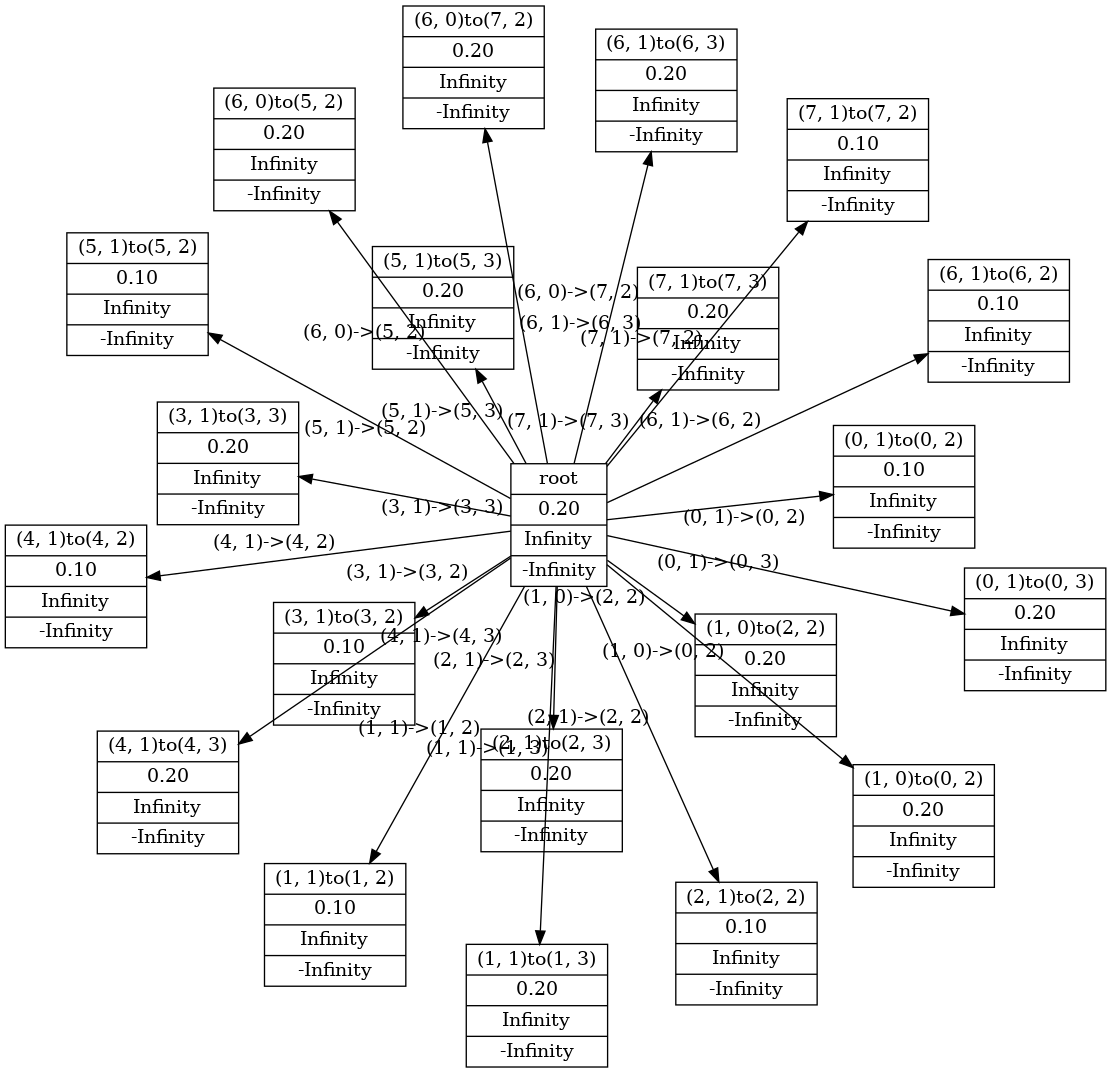
\includegraphics[width=0.7\textwidth]{out.png}
    \caption{Une image généré par le programme Graphviz.}
    \label{fig:graph-graphviz}
\end{figure}

\subsection{Nombreuses commandes disponibles avec UCI}
\par Le premier problème que on a rencontré pendant le développement est le problème de la réalisation d'une interface UCI. Au début de développement on a pas assez de connaissance sur le fonctionnement d'ARENA, ainsi que comment ce logiciel peut interagir avec le code Java. Ensuite on a trouvé le fichier qui décrit le protocole UCI\cite{doc:uci}. C'est un document daté de 2006 qui a proposé vingtaines commandes à traiter. Sûrement en réalisant toutes les commandes de façon robuste permet d'avoir un système de la meilleur fonctionnalité, mais on trouve après les essaies, alors que les commandes listées dans la section \ref{commandes} sont nécessaires pour un système basique. En donc on a choisi implémenter ces commandes.

\par D'ailleurs, grâce à l'implémentation du syntaxe \texttt{switch}, ce possible d'ajouter plus de commandes dans le programme plus tard sans modifier la structure du programme. 

\subsection{Problème avec l'exécution du code sur les plateformes Linux/Windows}
\par Le développement de ce programme est fait totalement sur un système Linux Ubuntu 22 LTS. La différence entre un système Linux et un système Windows normalement ne pose pas de problème, ceci dit, il y a une différence non négligeable c'est le traitement d'un fichier donné. Le système Windows connaît les suffixes dans le nom d'un fichier, et il fait le bon logiciel exécuter les opérations. Donc sur un système Windows, le fichier \texttt{.jar} est un format valid pour un engine d'échecs pour l'ARENA. Car en mettant le fichier dans une commande d'exécution, le code exécuté réellement est \texttt{java -jar xxx.jar}. Alors que sur un système Linux, la ligne de commande ne permet d'identifier un fichier \texttt{.jar}, ARENA ne peut pas "exécuter" un fichier de tel format.

\par Pour résoudre ce problème, la première solution qu'on a conçu est de retrouver un programme qui permet de compiler un fichier \texttt{.jar} et sortir un fichier exécutable. Malheureusement cette solution est difficile à cause de la manque de solution facile. Nous avons donc choisi une solution alternative : on a créé un programme C qui lance le fichier \texttt{.jar} en appelant la fonction \texttt{execvp}\cite{doc:evecvp}. Le programme C est disponible dans le listing \ref{lst:launcher}.

\par Un problème parasite est résolu avec la version de Java utilisé pour l'exécution. Le programme a été écrit avec une version récente de Java 19. Ainsi comment le fichier \texttt{.jar} a été généré. Il semble que le fichier \texttt{.jar} généré demande donc une version de Java VM assez récente pour son exécution ; il faut préciser dans la ligne de commande \texttt{--enable-preview} afin d'avoir le programme fonctionner. C'est la raison pourquoi que le programme a échoué son exécution pendant la petite compétition réalisée à l'UQAC le 22 novembre. Heureusement, après une réflexion, je pense que la configuration d'ARENA permet de l'ajout des paramètres dans la ligne de commande\footnote{Personnellement je n'ai pas encore testé son fonctionnalité sur un plateforme Windows, mais dans le pire cas le code Java est toujours disponible et vous pouvez faire la compilation à partir du code disponible sur \url{https://github.com/LuoQuestionmark/projet-ia-echecs}}.

\subsection{Optimisation avec le mouvement du "Roi"}\label{sect:bug}

\par La dernière changement que on a effectué sur le programme est une optimisation. Nous avons remarqué que la qualité de la solution retrouvée est influencée fortement par le profondeur de recherche. Pour gagner le temps à une exploration plus profonde, on a utilisé \texttt{VisualVM} pour obtenir le profil du programme. On a remarqué que le programme a passé le temps pour l'analyse du mouvement de la pièce "Roi", car dans la version précédente, on a considéré que cette pièce ne devrait pas être capable de déplacer vers une case qui peut être attaquée. La réalisation de cette méthode, demande finalement de calculer toutes les mouvements possibles des pièces de l'autre joueur\footnote{Techniquement pas tous les mouvements de leur "Roi", sinon il y aura une récursion infinie}. C'est donc un calcul très lourd. Après une réflexion, on a décidé de abandonner cette fonctionnalité, car théoriquement un système sain ne choisit pas le mouvement de "se suicider". Ce choix nous économise beaucoup de temps de calcul, permet de calculer maintenant un profondeur de 5 au lieu de 2.

\par Le changement introduit un nouveau problème, car maintenant l'engine ne peut pas retrouver le situation du pat\cite{frwiki:pat}. Mais on suppose que cette situation n'arrive pas souvent. Donc pour l'instant on le laisse dans notre programme.

\section{Conclusion}
\par Dans ce document, on a présenté le programme qu'on a réalisé pour ce projet d'intelligence artificielle, le fonctionnement de notre programme, leur implémentation, ainsi les problèmes, les solutions, et les réflexions qu'on a expérimenté pendant la réalisation de ce projet.

\par Le rendu de ce projet est donc ce document avec un engine d'échecs, nommé OCAP. Les commandes qu'il est capable à traiter ont été données dans la section \ref{commandes}, et un bug connu est discuté dans la section \ref{sect:bug}. Le code de source est disponible sur GitHub : \url{https://github.com/LuoQuestionmark/projet-ia-echecs}.

\par Personnellement je suis content que le projet est terminé sans trop de difficultés et je suis fié avec le programme que j'ai écrit.

\clearpage
\bibliographystyle{plain}
\bibliography{refs}

\clearpage
\begin{appendices}
\section{Code implémenté}

\begin{lstlisting}[language=java, caption={Une partie des fonctions réalisées dans la classe \texttt{Board}.}, label={lst:board}]
public class Board implements Cloneable {

    private final double heuristicConst = 0.1;

    private HashMap<PieceType, ArrayList<Piece>> availablePieces = new HashMap<>();
    private TreeMap<Coord, Piece> board = new TreeMap<>();

    private boolean isBlackMove = false;
    
    public Coord enpassant = null; // null means no "enpassant"
    // otherwise is the last coord of the "enpassant"
    // these variables are used to track the "castling"
    // zero for black, one for white
    private boolean[] isKingMoved = {false, false};
    private boolean[] isLeftRockMoved = {false, false};
    private boolean[] isRightRockMoved = {false, false};

    public boolean isBlackMove() {...}
    public TreeMap<Coord, Piece> getWhitePieces() {...}
    ...
}
\end{lstlisting}

\begin{lstlisting}[language=java, caption={La classe abstracte \texttt{Piece}.}, label={lst:piece}]
package Board;

import java.util.TreeSet;

import mUtil.Coord;

public abstract class Piece {
    protected boolean isBlackVal;
    abstract public TreeSet<Coord> getLegalMoves(Board currentBoard, Coord currentCoord);

    abstract public String getShortName();
        
    public Piece(boolean isBlack) {
        this.isBlackVal = isBlack;
    }
    
    public boolean isBlack() {
        return isBlackVal;
    }

}
\end{lstlisting}

\begin{minipage}{\linewidth}
\begin{lstlisting}[language=java, caption={La variable \texttt{isFinish} et son utilisation sur la synchronisation.}, label={lst:isFinish}]
synchronized public double explore(int depth, Node current) {
    // the actual recursive body of function "explore"
    if (this.isFinish || depth == 0) {
        return current.calScore(true);
    }
    
    double val;
    Board newBoard;
    Node child;
    synchronized (lock) {...}
}
\end{lstlisting}
\end{minipage}


\begin{lstlisting}[language=java, caption={La recherche récursive, réalisée par un thread séparant.}, label={lst:recherche}]

@Override
public void run() {
    int depth = 1;
    while (!isFinish && depth <= depthLimit) {
        explore(depth);
        depth += 1;
        System.out.format("info depth %d finish\n", depth);
        this.oldRoot = this.root;
        this.root = new Node(board);
    }
}
    
\end{lstlisting}

\begin{lstlisting}[language=java, caption={Le parseur qui traite les entrées.}, label={lst:parseur}]
private static void inputParser(String inputString) {
    String[] tokens = inputString.split("[ ]+");
    switch (tokens[0]) {
        case "uci":
            printUCI();
            break;
        case "isready":
            printIsReady();
            break;
        case "go":
            startAnalyser();
            break;
        case "stop":
            Move m = stopAnalyser();
            if (m == null)
                break;
            printBestMove(m);
            break;
        case "quit":
            if (notifier != null) {
                notifier.finish();
            }
            if (analyser != null) {
                analyser.finish();
            }
            System.exit(0);
            break;
        case "position":
            dealPosition(tokens);
            break;
        default:
            break;
    }
}
\end{lstlisting}

\begin{lstlisting}[language=java, caption={Le corps de la partie qui traiter les entrées/sorties.},label={lst:io}]
public static void main(String[] args) throws IOException {
    bufferedReader = new BufferedReader(new InputStreamReader(System.in));
    startReadInput();
    while (true) {
        try {
            Thread.sleep(timeout);
            if (analyser != null) {
                Move m = analyser.getBestMove();
                printBestMove(m);
            }
        } catch (InterruptedException e) {
            while (bufferedReader.ready()) {
                String line = bufferedReader.readLine();
                inputParser(line);
            }
        }
    }
}
    
\end{lstlisting}

\begin{lstlisting}[language=c, caption={Ce programme en C permet de lancer le fichier .jar par sa version compilée sur un système Linux.}, label={lst:launcher}]
#include <stdio.h>
#include <unistd.h>
#include <errno.h>
#include <string.h>

#define PATH_MAX 2000

extern int errno;

// java --enable-preview -jar projet-ia-echecs.jar 

int main(int argc, char** argv) {
    // chdir("./build");
    char cwd[PATH_MAX];
    char* args[] = {"java", "--enable-preview", "-jar", "./projet-ia-echecs.jar", NULL};
    execvp(args[0], args);
    perror("");
}
\end{lstlisting}

\end{appendices}

\end{document}
